\section{Programming paradigm}

Programming paradigms are derived from the way people perceive the real world, and programming languages are tools for formally describing this way of perception. When people develop software, they model the real world in a computer, and the different programming paradigms lie in the different ways of modeling the real world. Modeling the world often requires solving two problems. The first is to find out what the basic units of the world are, called first-class citizens. These first-class citizens can be stored in variables, passed as function parameters and function return values, in short, the "data" to be manipulated in a program. The second is to find out the relationship between these basic units, called computation. Computation can be seen as the "manipulation" of data in a program. For example, object-oriented treats objects as first-class citizens, and computations between objects are called methods. Another example is functional style, where functions are considered first-class citizens and computations are lambda calculations, which are computations on the functions themselves. Interestingly, functions in functional style are both the basic unit and the form of computation.

The programming paradigm is the lowest level of design for programming languages. Theoretically, programming languages need to help people to do the modeling of the real world, and therefore need to consider what modeling infrastructure should be provided, i.e., the programming paradigm of the programming language. Practically speaking, the design of a programming language should first consider the first-class citizen as the basic unit of the programming language. There is a certain conflict between different programming paradigms, stemming from the conflict of first-class citizens. In particular, it is very difficult to add a new paradigm to a programming language that defines the paradigm. A typical example is Java. the functional features added by Java8 do not fundamentally change the programming paradigm of Java, but are at best syntactic sugar. The lack of the original programming paradigm design makes it difficult for Java to be fully compatible with functional features, and thus the functional style in Java is crippled and inelegant. Therefore, for programming languages, especially for modern programming languages with multiple paradigms, the programming paradigm, and thus the first-class citizens, should be determined first.

Functional programming (FP) and object-oriented programming (OOP) are the two most common, and at the same time the most important, paradigms in modern programming languages. Therefore, these two paradigms are chosen for analysis when discussing programming paradigms below.

\subsection{Languages, paradigms, and concepts}

\begin{figure}[htbp]
    \centerline{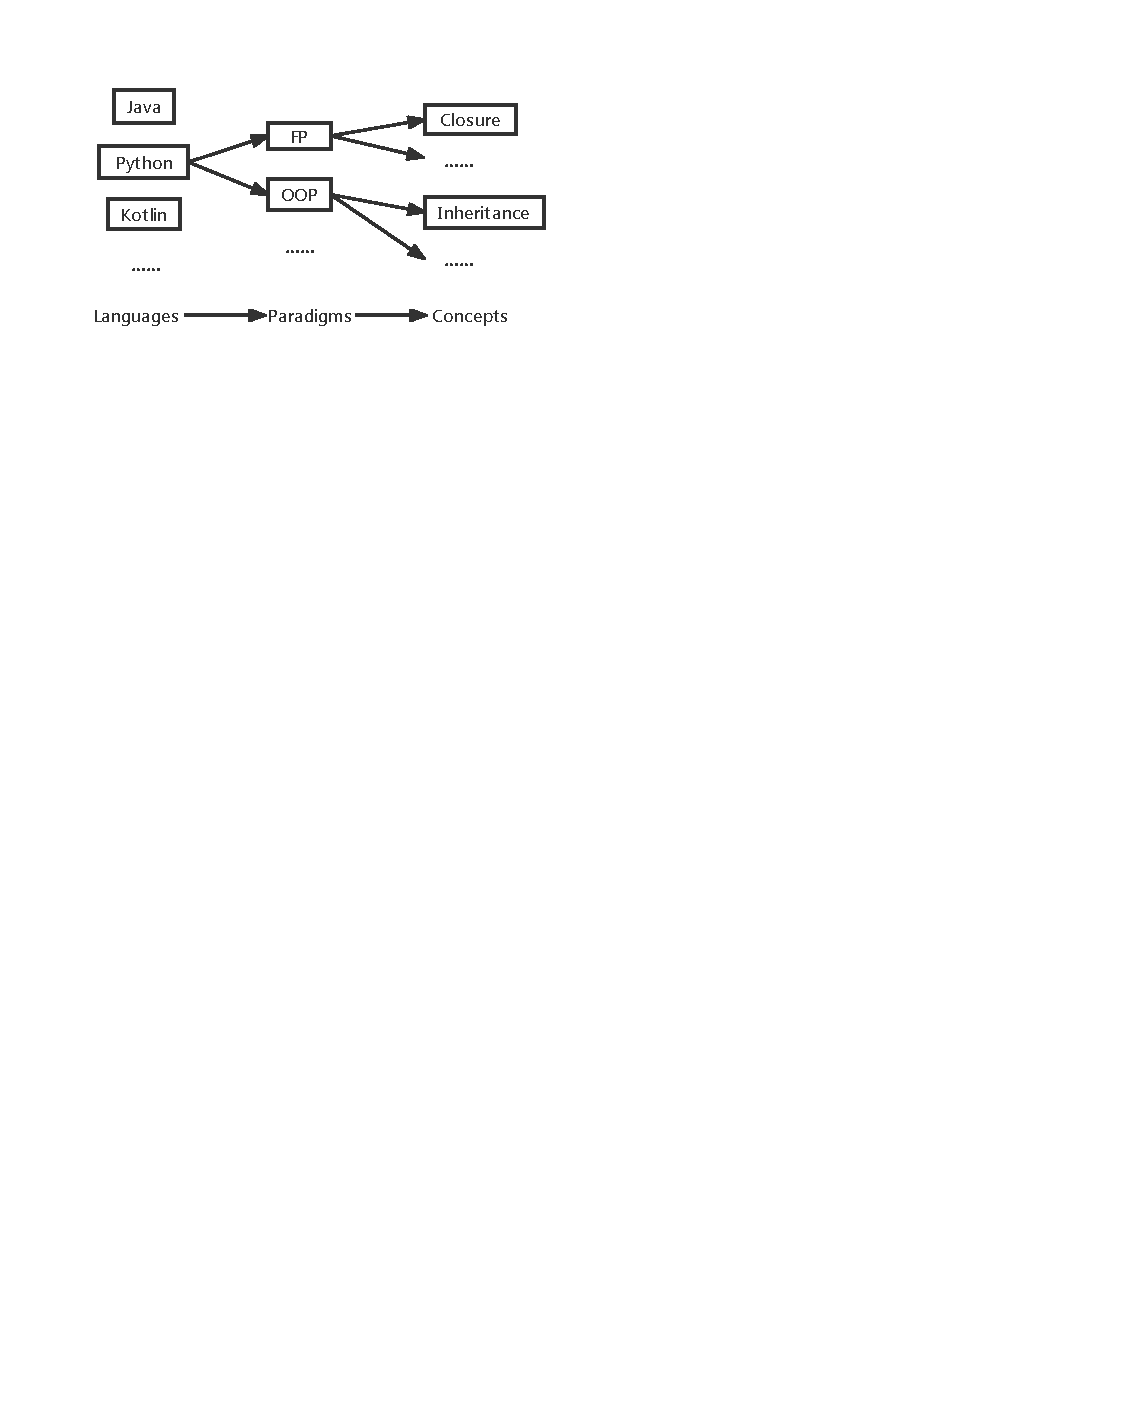
\includegraphics[scale=0.8]{figures/concept}}
    \caption{concept}
    \label{fig:concept}
\end{figure}

The diagram shows the relationship between languages, paradigms, and concepts. Each paradigm contains a core set of concepts, and at the same time, each language implements multiple paradigms. Functional and object-oriented are the programming paradigms typically found in modern programming languages. The degree of support for them varies across programming languages, and the table shows the degree of support for functional and object-oriented concepts in each language.

For the concepts that make up the programming paradigm, a more practically oriented organization is chosen here. It will favor the selection of concepts defined in specific programming languages rather than those defined in programming paradigm theory. For example, for the functional concept of nested and anonymous functions, they are implemented in many programming languages as lambda expressions. Another example is for the object-oriented concept of composition, which is supported by most of the currently popular programming languages. In fact, for programming language design itself, composition is simply a way of arranging data, it does not belong to any paradigm. Even languages like the more ancient one, C, provide structure combinations and function combinations. Therefore, it is not included in the analysis.

\begin{table*}[ht]
    \caption{concept}
    \label{tab:concept}
    \begin{center}
        \begin{tabular}{cll}
            \toprule
            Paradigm & Concept & Meaning \\
            \midrule
            FP & Higher-order functions & Take functions as variables, which can
            pass as parameters or return values. \\
            FP & Lambda expression & A short block of code which takes in parameters
            and returns a value. \\
            FP & Partial application & Given a function with certain parameters,
            producing another function (with fewer parameters). \\
            FP & Closures & A record stores a function together with an
            environment\cite{sussman1998scheme}. \\
            FP & Type inference & The automatic detection of the type of an
            expression at compile time. \\
            FP & Pattern matching & Dispatch branch by matching the pattern of a
            given sequence of tokens. \\
            FP & Statement as expression & Take all statements as expressions, which
            creates a definite value. \\
            OOP & Encapsulation & Hide the properties and implementation details of
            the object, and only expose the interface to the outside. \\
            OOP & Inheritance & Create classes that are built upon existing
            classes\cite{johnson1988designing}. A way of
            code reuse. \\
            OOP & Composition & Combine entities into more complex ones. A way of
            code reuse. \\
            OOP & Delegation & One entity passing something to another
            entity\cite{wilkinson2009grid}. A way of code
            reuse. \\
            OOP & Traits & A set of method conventions. Broadly including trait,
            interface, protocol and mixin. \\
            OOP & Polymorphism & Use of a single symbol to represent multiple
            different
            types\cite{cardelli1985understanding}. \\
            OOP & Everything is object & All the basic elements of a programming
            language are represented in the form of objects. \\
            \bottomrule
        \end{tabular}
    \end{center}
\end{table*}

\subsection{Functional programming}

The most important feature of functional programming is its high degree of abstraction. This is mainly because functional programming has its roots in the lambda calculus, so it has some of the characteristics of abstract algebra. In the practice of functional languages, the main idea is the combination and nesting of higher-order functions, so the core of its design is to sort out the rules of nesting and combination of higher-order functions. Therefore, the basic design method can be described as follows: through the standardization of the function transfer model and the combinability of higher-order functions, the description of the mapping of data from the source to the result is completed through a series of rule designs. The mapping here is accomplished by the formal combination of multiple higher-order functions. The description is like a mathematical formula that maps the input data into the result through layers of iterations. For the iterative process of data in a broad sense, this includes not only the iteration of the data itself, but also the iteration of the rules. This is due to the fact that in functional languages, data and rules are semantically unified in functions.

This leads to the characteristics of functional programming.

\begin{enumerate}
    \item High expressiveness. Functional programming is a data-driven expression with a high degree of abstraction, so that business logic can be accomplished with very little code within the scope of its expression.
    \item High maintainability within certain limits. First, functional programming is declarative expression and easy to understand. Second, higher-order functions are less granular and more composable. But its high maintainability is subject to certain conditions. First, the business logic is complex and not logically self-consistent in every aspect, so finding a complete set of rules to map is difficult. Second, both the rules of mapping are found in a narrow domain, but once it needs to be expanded to a new domain, the original rules will fail.
    \item High reliability. Since functional languages are based on lambda calculus, formal verification of functional code is relatively easy. Thus correctness and reliability can be guaranteed.
    \item Poor performance on Turing machines. In functional languages, there are more intermediate layers between the syntax rules and the Turing machine, as well as its syntax rules and inert evaluation, which makes optimization more difficult.
\end{enumerate}

\begin{table*}[ht]
    \caption{fp}
    \label{tab:fp}
    \begin{center}
        \begin{tabular}{cccccccc}
            \toprule
            Language & Higher-order functions & Lambda expression & Partial
            application & Closures & Type inference & Pattern matching & Statements
            as expressions\\
            \midrule
            Python     & \Checkmark & \Checkmark & Python2.5   & \Checkmark & \Checkmark & Python3.10  & ×          \\
            Java       & Java8      & Java8      & Java8       & Java8      & Java10     & ×           & ×          \\
            C++        & C++11      & C++11      & C++11       & C++11      & C++11      & C++17       & ×          \\
            JavaScript & \Checkmark & \Checkmark & ECMAScript5 & \Checkmark & \Checkmark & ECMAScript6 & ×          \\
            Go         & \Checkmark & \Checkmark & \Checkmark  & \Checkmark & \Checkmark & ×           & ×          \\
            Swift      & \Checkmark & \Checkmark & \Checkmark  & \Checkmark & \Checkmark & \Checkmark  & ×          \\
            Dart       & \Checkmark & \Checkmark & \Checkmark  & \Checkmark & \Checkmark & ×           & ×          \\
            Rust       & \Checkmark & \Checkmark & \Checkmark  & \Checkmark & \Checkmark & \Checkmark  & \Checkmark \\
            Kotlin     & \Checkmark & \Checkmark & \Checkmark  & \Checkmark & \Checkmark & \Checkmark  & \Checkmark \\
            \bottomrule
        \end{tabular}
    \end{center}
\end{table*}

As programming language practice has deepened, programming languages have become more and more supportive of functional concepts. With for the programming languages released in the 1980s and 1990s, the support for functional style was not good when programming languages were first created. In particular, Java and C++, from their initial syntax, were not designed with functional programming in mind. This is better for JavaScript and Python, which inherently support functional style, but still lack some advanced functional concepts. For programming languages released around 2010, the basic concepts of functionalism are supported. Rust and Kotlin, in particular, additionally support the concept of "Statements as expressions", a milestone in the development of modern programming language paradigm convergence. The concept of "statements as expressions", which is more common in functional languages, enables semantic unification of expressions and statements, but is not implemented in most programming languages that integrate object-oriented and functional paradigms. As programming languages continue to evolve, Kotlin and Rust have implemented a fusion of functional and object-oriented paradigms that includes this concept, so Kotlin and Rust can be considered as functional paradigms with a higher level.

\subsection{Object oriented orogramming}

The most important feature of object orientation is the emphasis on reuse. Back in the 1960s, software maintenance became increasingly difficult due to the increasing complexity of software and hardware. Object-Orientation solves this problem by emphasizing reusability. In the practice of object-oriented languages, people mapped real problems into entities and their relationships, rather than caring about the process of dealing with the problem. After the birth of object-oriented languages, there was an urgent need for a modeling approach that mapped problems into entities and relationships, at which point UML was born. It is a standardized modeling language consisting of a set of icons that has greatly contributed to the development of object-oriented methodologies. This approach emphasizes the importance of modeling and design.


In the same way, the characteristics of object-oriented programming can be obtained.

\begin{enumerate}
    \item A certain expressiveness. While encapsulation increases the level of code abstraction, it essentially shifts and splits the business logic. In addition, the complex hierarchical structure of object-oriented reduces its expressiveness. Design patterns emerge to compensate for the shortcomings of object-oriented expression.
    \item High maintainability. First, the object itself is highly reusable and applicable to more areas. Second, polymorphism improves the ability to respond to change. Third, encapsulation facilitates the cost of understanding for maintainers.
    \item A certain degree of reliability. Object-oriented modeling relies on practical experience and lacks rigorous theoretical proof. The usual best practices for object-oriented modeling are limited to the realm of inductive methods.
    \item Better performance. Object-oriented can achieve near-native performance of Turing machines. Most of the performance overheads, such as dynamic binding, function call overheads, can be optimized by compilation means.
\end{enumerate}


And there is not much difference in the level of support for the core object-oriented concepts in popular languages. Because of their long history of development and no major theoretical or practical innovations in recent years, most programming languages have implemented the core object-oriented concepts relatively completely. In addition, more and more programming languages are implementing object-oriented features by supporting combinations and delegates, while mere inheritance has proven to be bad practice. As a result, the concepts of classes and inheritance have been abandoned in Go and Rust, and traditional object-orientation is implemented through trait. Compared to class-based object-orientation, trait-based object-orientation is more loosely coupled and more flexible to implement. However, most languages support both trait and class to enable different granularity of control.

To more accurately distinguish the strengths and weaknesses of each language's object-oriented programming paradigm, some less common concepts are introduced here. One example is "everything is object". According to the definition of object-oriented, it should have been the core concept in object-oriented. But in fact, early programming languages tended to have a lot of imperative features, and not all elements of a programming language were treated as objects. For example, there are still "primitive data types" in Java, which are not objects, so we cannot call methods of these types as if they were objects. There may be many performance positives of "primitive data types", but from a semantic consistency point of view, "primitive data types" have a negative effect. Therefore, languages with the concept of "everything is object" are considered to have better object-oriented features.

\begin{table*}[ht]
    \caption{oop}
    \label{tab:oop}
    \begin{center}
        \begin{tabular}{cccccc}
            \toprule
            Language & Inheritance & Delegation & Traits & Polymorphism &
            Everything is object \\
            \midrule
            Python     & \Checkmark & \Checkmark & ×          & \Checkmark & \Checkmark \\
            Java       & \Checkmark & ×          & \Checkmark & \Checkmark & ×          \\
            C++        & \Checkmark & ×          & \Checkmark & \Checkmark & ×          \\
            JavaScript & \Checkmark & \Checkmark & ×          & \Checkmark & \Checkmark \\
            Go         & ×          & ×          & \Checkmark & \Checkmark & ×          \\
            Swift      & \Checkmark & ×          & \Checkmark & \Checkmark & \Checkmark \\
            Dart       & \Checkmark & ×          & ×          & \Checkmark & \Checkmark \\
            Rust       & ×          & \Checkmark & \Checkmark & \Checkmark & \Checkmark \\
            Kotlin     & \Checkmark & \Checkmark & \Checkmark & \Checkmark & \Checkmark \\
            \bottomrule
        \end{tabular}
    \end{center}
\end{table*}

\subsection{Programming Paradigms and Applications}

\begin{figure}[htbp]
    \centerline{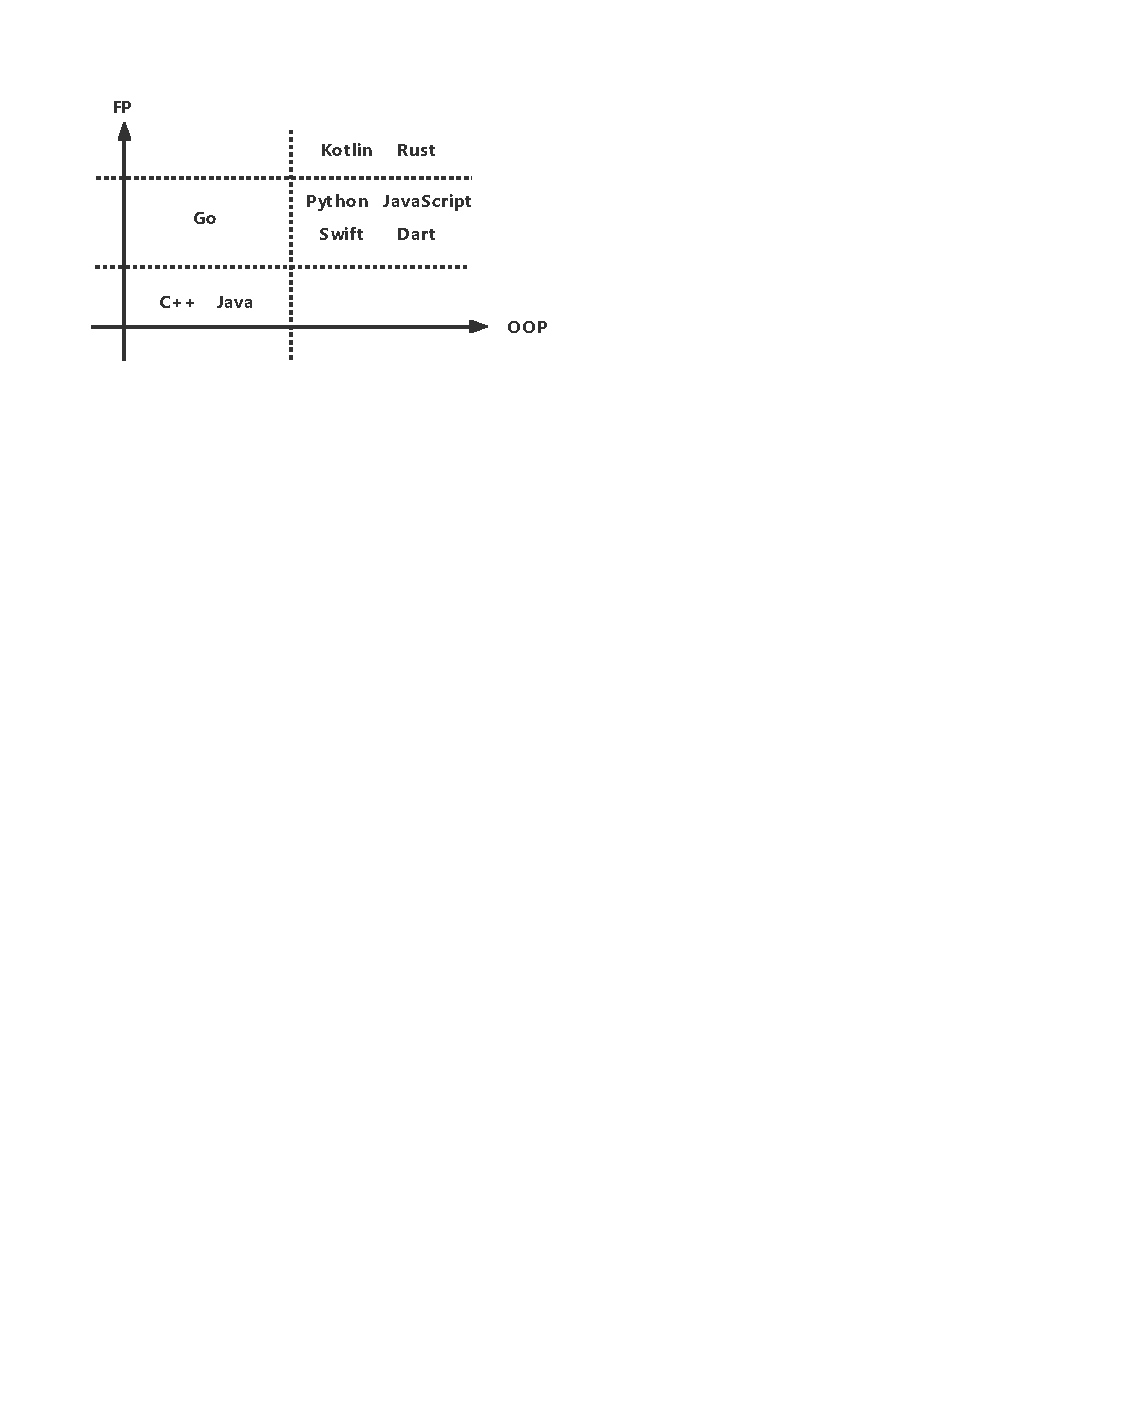
\includegraphics[scale=0.8]{figures/paradigm}}
    \caption{paradigm}
    \label{fig:paradigm}
\end{figure}

The above discussion leads to a diagram that roughly depicts the degree of support for functional and object-oriented programming concepts in different programming languages. For a given programming language, the closer it is to FP/OOP in the graph, the better it supports FP/OOP. In fact, the paradigm of a programming language is very closely related to its application scenario, whether it is for a single application area or for multiple application areas.

A typical example is Dart, whose main application scenario is the web front-end, often as a support language for the GUI framework Flutter. It is obvious that most of the GUI frameworks we use have a complex inheritance structure. This is because, for GUIs, most application scenarios satisfy the Richter substitution principle, i.e., the child type can completely replace the husband type. This is a sufficient condition for using inheritance. Therefore, Dart simply provides an object-oriented concept based on inheritance.

Another example is Java, which has weaker support for both FP and OOP concepts.Java was used for Enterprise development in the early years and provided an object-oriented paradigm in order to improve code reusability. Later it was used for Web servers, which had high requirements for abstraction of business logic, so the concept of functionalism was added additionally. But because of the historical legacy, the level of support is not good.

Another example is Kotlin, which has better support for both FP and OOP. Its initial application scenario was Android. To solve the traditional Java development Android code redundancy problem, Kotlin was designed to add a lot of functional and object-oriented concepts for the Android application scenario. These beneficial features allow Kotlin to be used in other scenarios, such as server front-ends and back-ends.

